%!TEX root = ..\Master.tex

\subsection{Artificial Neural Network}
Artificial neural networks are an attempt at creating a modelling how a brain works.
A network consists of neurons connected together. 
A neuron takes zero or more inputes, does some computation and gives one input as seen on figure \ref{fig:neuron}.

\begin{figure}[H]
\centering
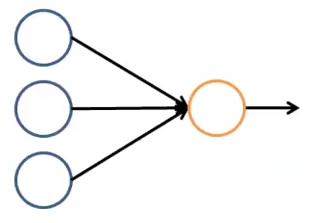
\includegraphics[scale=.5]{billeder/neuron}
\caption{A single neuron. The 3 blue circles are input units. The orange circle is the neuron.}
\label{fig:neuron}
\end{figure}

Neurons can be combined into networks as seen on figure \ref{fig:neural-network}.
How the neurons are connected is called the network architecture.
The first layer is called the input layer.
The last layer is called the output layer.
All other layers are called hidden layers.
The nodes in the network are called units.

The network on figure \ref{fig:neural-network} has 3 input units and 1 output unit which in machine learning terms means it takes 3 features and does binary classification.
To do multi-class classification, the output layer shall contain one output unit per class.

\begin{figure}[H]
\centering
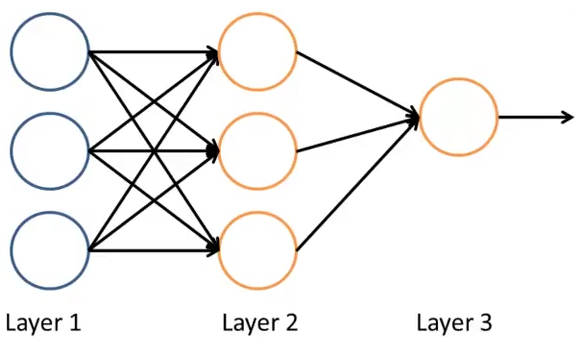
\includegraphics[scale=.5]{billeder/neural-network}
\caption{An artificial neural network with 3 layers.}
\label{fig:neural-network}
\end{figure}

Neural networks can be thought of as an extension of logistic regression.
In logistic regression we would only have layer 2 and 3, where layer 2 would contain the features.
In neural networks we can add more layers, where each new layer maps the features of the previous layer to a set of new features.
This gives more flexibility and expressive power in the model.

\subsubsection{Mathematical representation}

$a_i^{(j)}$ is the activation of unit $i$ in layer $j$, which uses the Sigmoid activation function: 
\begin{equation}
a(x) = \dfrac{1}{1+e^{-{\Theta}^Tx}}
\end{equation}
$\Theta^{(j)}$ is a matrix of weights, controlling function mapping from layer $j$ to layer $j+1$.
If the network has $s_j$ units in layer $j$ and $s_{j+1}$ units in layer $j+1$, then $\Theta^{(j)}$ will be of dimension $s_{j+1}\times(s_j+1)$.
Each layer also contains a bias unit $a_0^{(j)}$.
The representation is illustrated on figure \ref{fig:neural-network-detailed}.


\begin{figure}[H]
\centering
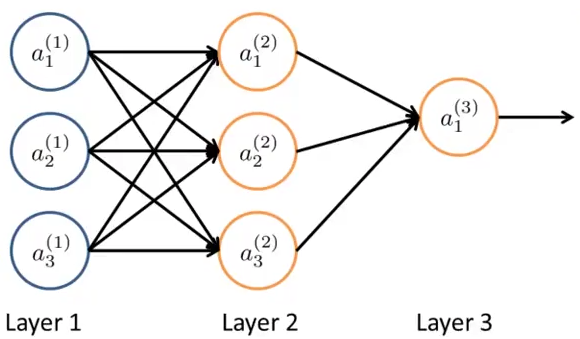
\includegraphics[scale=.5]{billeder/neural-network-detailed}
\caption{An artificial neural network with 3 layers.}
\label{fig:neural-network-detailed}
\end{figure}

The activation of a layer is defined as:

\begin{equation}
a^{(j+1)} = g(\Theta^{(j)}a^{(j)})
\end{equation}

The activation of a layer is therefore dependant on the activation of the previous layer. So you have to start by activating the first layer and then propagate through the layers, hence the name of the algorithm; "forward propagation algorithm".

We can now compute the layer activations one at a time to get the output of the network on figure \ref{fig:neural-network-detailed}:
\begin{equation}
a^{(2)} = g(\Theta^{(1)}a^{(1)})
\end{equation}

\begin{equation}
a^{(3)} = g(\Theta^{(2)}a^{(2)}) = g(\Theta^{(2)} g(\Theta^{(1)}a^{(1)}))
\end{equation}

The activation of the output layer is also called:
\begin{equation}
h_\Theta(x) = a^{(3)}
\end{equation}

\subsubsection{Training the network}
Given $m$ training examples $\left\{(x^{(1)},y^{(1)}), (x^{(2)},y^{(2)}),\dots, (x^{(m)},y^{(m)}) \right\}$.
Training the neural network is an optimization problem, where a cost function $J(\Theta)$ should be minimized with respect to the weights $\Theta$:
\begin{equation}
\min_{\Theta} J(\Theta)
\end{equation}

We can minimize the cost function using an optimization algorithm like gradient descent. For such an optimization algorithm, we also need the partial derivatives of the cost funtion:
\begin{equation}
\frac{\delta}{\delta\Theta^{(l)}_{ij}}J(\Theta)
\end{equation}

The cost function $J$ is defined as:
\begin{equation}
\begin{split}
J(\Theta) = &-\frac{1}{m}
\left[
\sum^m_{i=1}\sum^K_{k=1}
y_k^{(i)}
log(h_\Theta(x^{(i)}))_k +
(1-y_k^{(i)})
log(1-(h_\Theta(x^{(i)}))_k)
\right] \\
&+ \frac{\lambda}{2m}
\sum^{L-1}_{k=1}
\sum^{s_l}_{i=1}
\sum^{s_{l+1}}_{j=1}
(\Theta^{(l)}_{ji})^2
\end{split}
\end{equation}

Where $L$ is the total number of layers, $s_l$ is the number of units in layer $l$, $K$ is the number of output units and $m$ is the number of training examples. The second term of the cost function is the regularization term. The regularization term is a extra condition added that guards the model against over fitting. It is a sum of the squares of all the weights in the network. This is scaled by a factor $\lambda/2m$, where $\lambda>0$ is known as the regularization parameter, and $m$ is, as usual, the size of our training set. When $\lambda$ is small we prefer to minimize the original cost function, but when $\lambda$ is large we prefer small weights.
\\\ \\
To find the partial derivatives, we can use the backpropagation algorithm:

The error term of the output layer is defined as:
\begin{equation}
\delta^{(L)} = a^{(L)}-y
\end{equation}

The error term of the hidden layers is defined as:
\begin{equation}
\delta^{(l)} = (1-a^{(l)})\Theta^{(l)}\delta^{(l+1)}
\end{equation}

There is no error term of the input layer. The partial derivative can then be found as:

\begin{equation}
\frac{\delta}{\delta\Theta^{(l)}_{ij}}J(\Theta) = 
\delta^{(l)}a^{(l)}
\end{equation}

In the speech recognition case, a artificial neural network have been trained to separate the data in the three classes. Before the neural network can be trained, must the number of hidden for a optimal fit be found. This is done by an exhaustive search. This is seen in figure \ref{fig:NNsearch}, where alpha is the regularization parameter.

\begin{figure}[H]
\centering
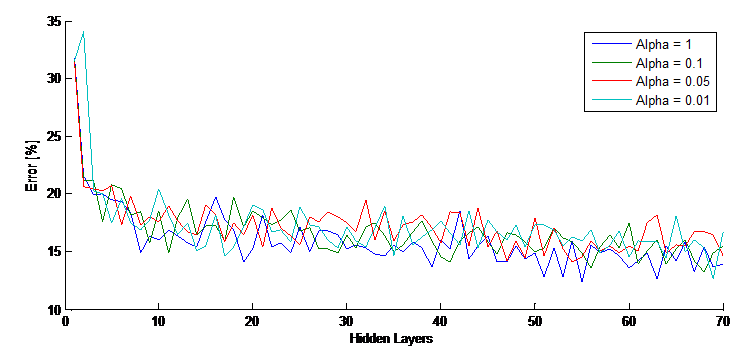
\includegraphics[scale=0.6]{billeder/TraningErrorNN}
\caption{Artificial neural network Exhaustive Search}
\label{fig:NNsearch}
\end{figure} 

It is found that 55 hidden state is the optimal number of hidden numbers. After training this network for a series of times to find the global minimum, separation is possible with a 12.4\%. This can be seen in the confusion matrix: 

\begin{figure}[H]
\centering
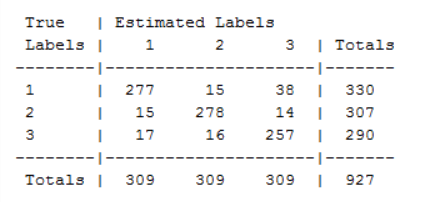
\includegraphics[scale=0.8]{billeder/conmatnn}
\caption{Confusion matrix for the artificial neural network }
\label{fig:conmatnn}
\end{figure}
%------------------------------------------------